%%%%%%%%%%%%%%%%%%%%%%%%%%%%%%% Inciso 01B:
\newpage
$b$) \begin{lstlisting}
  {with {a { - 5 5 } }
    {with {b { - a a } }
      {with {foo { fun {x} {- a b } } }
        {with {a {+ -3 -3 } }
          {with {b {+ a a } }
            {foo } } } } }
\end{lstlisting}

Primero construyamos las pilas de ambientes, con
respecto al régimen de evaluación, esto es 

%%%%%%%%%%%%%%%%%%%%%%  Glotona      %%%%%%%%%%%%%%%%%%%%%%%%%%%%
$*$) Con evaluación glotona:
  \begin{center}
    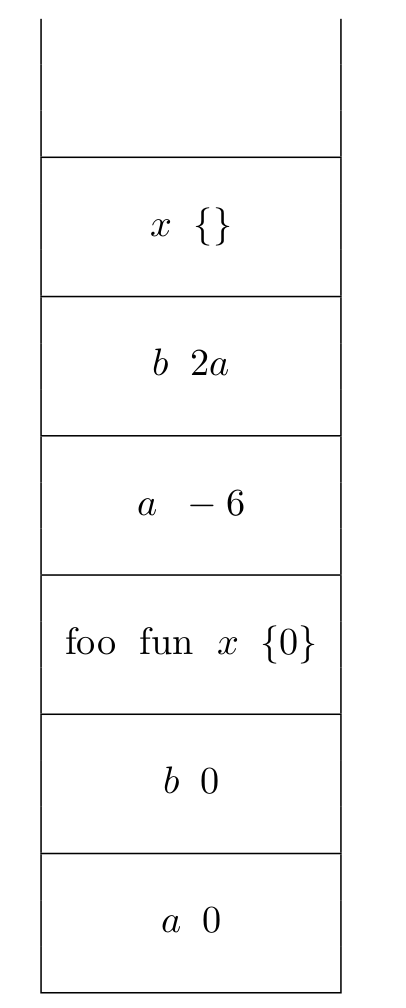
\includegraphics[scale=0.3]{./GlotonaB}
  \end{center}

\begin{enumerate}
  \item Evaluación glotona y alcance estático.
  \begin{lstlisting}
  {foo }
  {foo {}{-a b}}
  {foo {}{-a (0)}}
  {foo {}{-(0) (0)}}
  {-(0) (0)}
  {0}
  = 0
\end{lstlisting}
  \item Evaluación glotona y alcance dinámico.
  \begin{lstlisting}
  {foo }
  {foo {}{-a b}}
  {foo {}{-(-6) (-12)}}
  {-(-6) (-12)}
  {6}
  = 6
\end{lstlisting}

%%%%%%%%%%%%%%%%%%%%%%  Perezosa      %%%%%%%%%%%%%%%%%%%%%%%%%%%%
$*$) Con evaluación perezosa:
  \begin{center}
    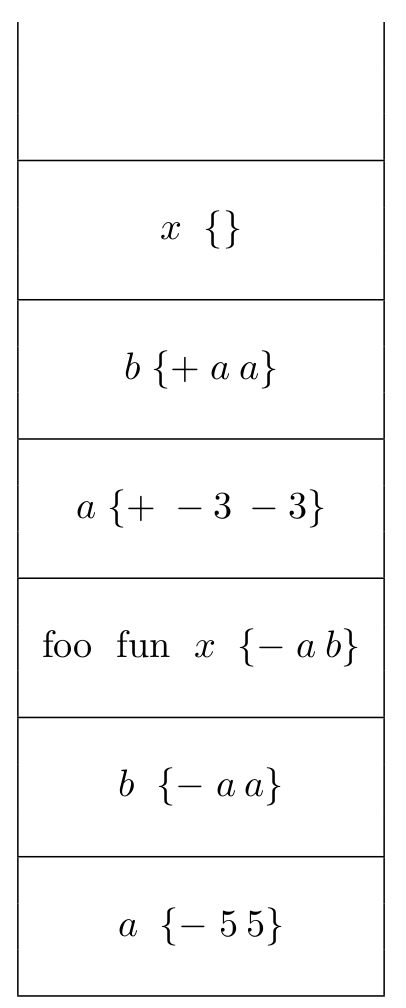
\includegraphics[scale=0.3]{./PerezosaB}
  \end{center}

\item Evaluación perezosa y alcance estático.
  \begin{lstlisting}
  {foo }
  {foo {}{-a b}}
  {foo {}{-a (-a a)}}
  {foo {}{-(-5 5) (-a a)}}
  {foo {}{-(-5 5) (-(-5 5) a)}}
  {foo {}{-(-5 5) (-(-5 5) (-5 5))}}
  {foo {}{-(-5 5) (-(-5 5) (0))}}
  {foo {}{-(-5 5) (-(0) (0))}}
  {foo {}{-(0) (-(0) (0))}}
  {foo {}{-(0) (0)}}
  {-(0) (0)}
  {0}
  = 0
\end{lstlisting}
  \item Evaluación perezosa y alcance dinámico.
  \begin{lstlisting}
  {foo }
  {foo {}{-a b}}
  {foo {}{-a (+a a)}}
  {foo {}{-(+ (-3) (-3)) (+a a)}}
  {foo {}{-(+ (-3) (-3)) (+ (+ (-3) (-3)) a)}}
  {foo {}{-(+ (-3) (-3)) (+ (+ (-3) (-3)) (+ (-3) (-3)))}}
  {foo {}{-(+ (-3) (-3)) (+ (-6) (-6))}}
  {foo {}{-(-6) (+ (-6) (-6))}}
  {foo {}{-(-6) (-12)}}
  {-(-6) (-12)}
  {6}
  = 6


\end{lstlisting}
\end{enumerate}
